\label{section:outputs}
\setcounter{footnote}{0}
\section{Outputs}

A Stockholm alignment file can include several different multiple
sequence alignments (MSAs).  For each alignment file
rnafile.sto, \rscape\ produces the following output files, one for
each individual alignment in an input Stockholm file:

\begin{sreitems}{\emprog{rnafile\_msaname.sorted.cov}}
%
\item[\emprog{rnafile\_msaname.cov}] Tabular output with the significant pairs,
  with their score and E-value, estimated number of substitutions and power.
%
\item[\emprog{rnafile\_msaname.sorted.cov}] Tabular output sorted from highest to
  lowest E-value.
%
\item[\emprog{rnafile\_msaname.power}]
Tabular output with the list of basepairs in the proposed RNA structure annotated their power. The file also reports 
the alignment power, and the expected number of basepairs to covary.
%
\end{sreitems}

\subsection{Covariation tabular output}

The distribution includes in the directory tutorials/ examples of
output files. If you run \rscape, the outputs will go into your
current working directory (not necessarily tutorials/).


The output file \emprog{tutorial/updated\_Arisong\_1.cov} looks like this:\\
\user{more tutorial/updated\_Arisong\_1.cov}

\begin{sreoutput}
# Method Target_E-val [cov_min,cov_max] [FP | TP True Found | Sen PPV F] 
# GTp    0.05           [-9.78,121.66]    [0 | 11 20 11 | 55.00 100.00 70.97] 
#
# in_given  left_pos       right_pos        score          E-value       substitutions      power
#-------------------------------------------------------------------------------------------------------
*               94             110      57.27959        0.00760538      37              0.40
*               96             108      88.43400        0.000466924     26              0.28
...
\end{sreoutput}
The output file is a tabular list of significant pairs sorted by sequence positions:

\begin{sreitems}{\prog{Second and third columns}}
 \item[\prog{First column}] indicates whether the significant pair is
   part of the given structure (*), or not.  If the pair is not in the
   structure, we distinguish whether the pair is compatible with the
   given structure ($\sim$) or not (blank).

  In addition, if the structure is provided by a PDB file (using the
  option \prog{--pdb}), a non Watson-Crick/Watson-Crick base pair
  is designated by ``**''. A contact that is not a basepair is
  designated by: ``$c\sim$'' if compatible with all the basepairs, or
  by ``$c$'' otherwise.

 \item[\prog{Second and third columns}] are the two positions of the
   pair, $i\leq j$ respectively. Positions are relative to the input
   alignment.

 \item[\prog{Fourth column}] is the covariation score.

 \item[\prog{Fifth column}] is the E-value. Significant positions
   have E-values $<< 1$.

 \item[\prog{Sixth column}] is the estimated number of total substitutions in the two columns.
 
 \item[\prog{Seventh column}] is the basepair power or probability that it should covary.
 
 \end{sreitems}
 The output file also includes two comment lines per alignment in the
 file:

 \begin{sreitems}{\prog{Second comment line}} \item[\prog{First
 comment line}]describes properties of the alignment: number of
 sequence (nseq), alignment length (alen), average percentage identity
 (avgid), and number of base pairs (nbpairs).  Values in parentheses
 correspond to the alignment as given. Values not in parentheses
 correspond to the analyzed alignment after the filters (for redundant
 sequences and gapped columns) have been applied.

 \item[\prog{Second comment line}]describes properties of the \rscape\
   search: the covariation method (GTp), the E-value threshold (0.05),
   the range of scores for all pairs in the alignments (from -9.7 to
   89.1), the number of covarying non base pairs (0), the number of
   covarying base pairs (11), the number of base pairs (20), and the
   total number of covarying pairs (11). Lastly we provide the
   sensitivity (SEN=55.00=11/20), positive predictive value
   (PPV=100.00=11/11), and F-measure (F=70.97 = 2 * SEN * PPV /
   (SEN+PPV)).  \end{sreitems}

\subsection{Power tabular output}
The output file \emprog{tutorial/updated\_Arisong\_1.power} looks like this:\\
\user{more tutorial/updated\_Arisong\_1.power}

\begin{sreoutput}
# Power analysis of given structure 
#
# covary  left_pos      right_pos    substitutions      power
#----------------------------------------------------------------
     *    94            110             37              0.40
          95            109             28              0.31
     *    96            108             26              0.28
     *    97            107             58              0.59
     *    98            106             45              0.48
     *    99            105             15              0.14
          100           104             20              0.21
.
.
.
     *    122           137             57              0.58
     *    123           135             72              0.68
     *    124           134             20              0.21
          125           133             31              0.34
#
# BPAIRS 20
# avg substitutions per BP  43.7
# BPAIRS expected to covary 8.3
# BPAIRS observed to covary 11
\end{sreoutput}
%
This file includes the list of all basepairs in the proposed structure
given with the input alignment. Each basepair is annotated with the
estimated number of substitutions and power.

\subsection{Default graphical outputs}
By default, the following files are also produced

\begin{sreitems}{\emprog{rnafile\_msaname.R2R.sto.\{pdf,svg\}}}
\item[\emprog{rnafile\_msaname.R2R.sto}] Stockholm file annotated by a
  modified version of the R2R program. This file includes the
  information necessary to draw the consensus structure, and to
  annotate the significantly covarying base pairs.
%
\item[\emprog{rnafile\_msaname.R2R.sto.\{pdf,svg\}}] Drawing of the
  \rscape-annotated consensus secondary structure.
%
\item[\emprog{rnafile\_msaname.surv}] A two column file with the 
survival functions (surv) for the covariation scores.
%
\item[\emprog{rnafile\_msaname.surv.ps}] Plot of the score's survival function
$P(X > \mbox{score})$. Drawing this
file requires that program \emprog{gnuplot} is installed somewhere in
the
\prog{\$\{PATH\}}, or that the environmental variable GNUPLOT 
pointing to a gnuplot executable is defined.
%
\item[\emprog{rnafile\_msaname.dplot.\{ps,svg\}}] Dot plot of the consensus
  secondary structure annotated according to covariation. Drawing of this
file requires that program \emprog{gnuplot} is installed somewhere in the
\prog{\$\{PATH\}}, or that the environmental variable GNUPLOT 
pointing to a gnuplot executable is defined.
%
\end{sreitems}
For each alignment, \emprog{msaname} is given
by \prog{<ACC>\_<ID>}, the combination of the accession \prog{\#=GF
AC <ACC>} and name \prog{\#=GF ID <ID>} in the Stockholm-format markups (or
one of two if the other in not defined).  If none of those fields are
defined, \emprog{msaname} is a number describing the order in the
file of the given alignment.

\subsection{Details about graphical outputs}
 Two files are produced per alignment in the input file: \\

 File \emprog{tutorial/updated\_Arisong\_1.R2R.sto} is a Stockholm
 formatted alignment that includes the input alignment annotated with
 the consensus structure. This Stockholm file also includes the
 additional annotation required to use the drawing program R2R.

 It is possible that the resulting drawing will show parts of the
 secondary structure occluded from each other (especially for long
 RNAs).  Using this file, one can customize a different drawing of the
 structure using the R2R documentation, provided in
 \prog{lib/R2R/R2R-manual.pdf}.\\

 File \emprog{tutorial/updated\_Arisong\_1.R2R.sto.pdf} depicts the
 consensus structure with the R-scape covariation annotation using the
 R2R software to depict the alignment.  The defaults used by R-scape
 to depict the alignment positions are given in this legend,

\begin{figure}[h]
   \begin{center}
   \includegraphics[scale=0.9]{R2Rlegend.png} 
  \end{center}
\end{figure}
 
 File \emprog{tutorial/updated\_Arisong\_1.surv} looks like this:

\user{more tutorial/updated\_Arisong.surv}
 \begin{sreoutput}
121.795428      0.05
95.862635       0.1
89.113004       0.15
...
 &
63.890698       0.000485437
58.917286       0.000970874
47.904730       0.00145631
...
 &
81.652885       2.40385e-06
77.745204       4.80769e-06
77.034717       7.21154e-06
...
 &
256.788050      2.64342e-17
256.432807      2.7899e-17
256.077563      2.94449e-17
...
 &
 \end{sreoutput}
 The first column is a covariation score (x). The second column is the
 survival function $P(X > x)$, that is the frequency of pairs having
 score larger than x. The file includes four survival functions separated by a
 ``\&'' line. The three survival functions correspond to:

 \begin{sreitems}{\prog{Second function:}}
 \item[\prog{First functions:}] the given alignment, proposed base pairs.
 (This section is empty if no secondary structure is proposed.)
 \item[\prog{Second functions:}] the given alignment, not proposed pairs.
 \item[\prog{Third function:}] the aggregation of all null alignments, all possible pairs.
 \item[\prog{Fourth function:}] the expected null survival function according to the tail Gamma fit.
 \end{sreitems}

\subsection{Using option --cacofold}
If the option \prog{--cacofold} is used, \rscape\, produces the
following additional files describing the maximal-covariation optimal
secondary structure:

\begin{sreitems}{\emprog{rnafile\_msaname.fold.R2R.sto.\{pdf,svg\}}}
\item[\emprog{rnafile\_msaname.fold.sto}]
The original alignment with the R-scape structural annotation 
%
\item[\emprog{rnafile\_msaname.fold.R2R.sto}]
File used by R2R to display the R-scape structure
%
\item[\emprog{rnafile\_msaname.fold.R2R.sto.\{pdf,svg\}}]
%
\item[\emprog{rnafile\_msaname.fold.surv}]
%
\item[\emprog{rnafile\_msaname.fold.surv.\{ps.svg\}}]
%
\item[\emprog{rnafile\_msaname.fold.dplot.\{ps,svg\}}]
%
\end{sreitems}
These files are formatted identically to those describing the given
consensus structure.


\clearpage
\subsection{Graphical outputs per alignment}
 Three plots are produced per alignment in the input file: 

 \begin{figure}[h]
   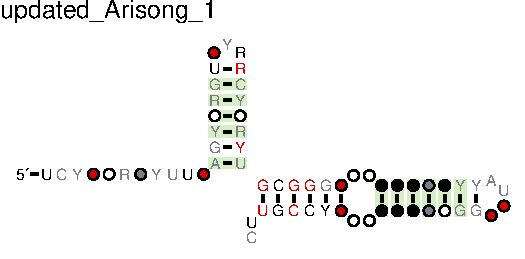
\includegraphics[scale=1.5]{Arisong_R2R.pdf} 
 \caption{\small\textbf{\emprog{tutorial/updated\_Arisong\_1.R2R.sto.\{pdf,svg\}}:
     annotated consensus secondary structure.} Base pairs with
   covariation scores equal or below the target E-value (0.05 as
   default) are depicted in green. By default only positions in the
   alignment with more than 50\% occupancy are depicted (unless they form
   a base pair). Option \prog{--r2rall} forces the depiction of all
   positions in the alignment.  }
 \label{fig:r2r}
 \end{figure}

 \begin{figure}[h] 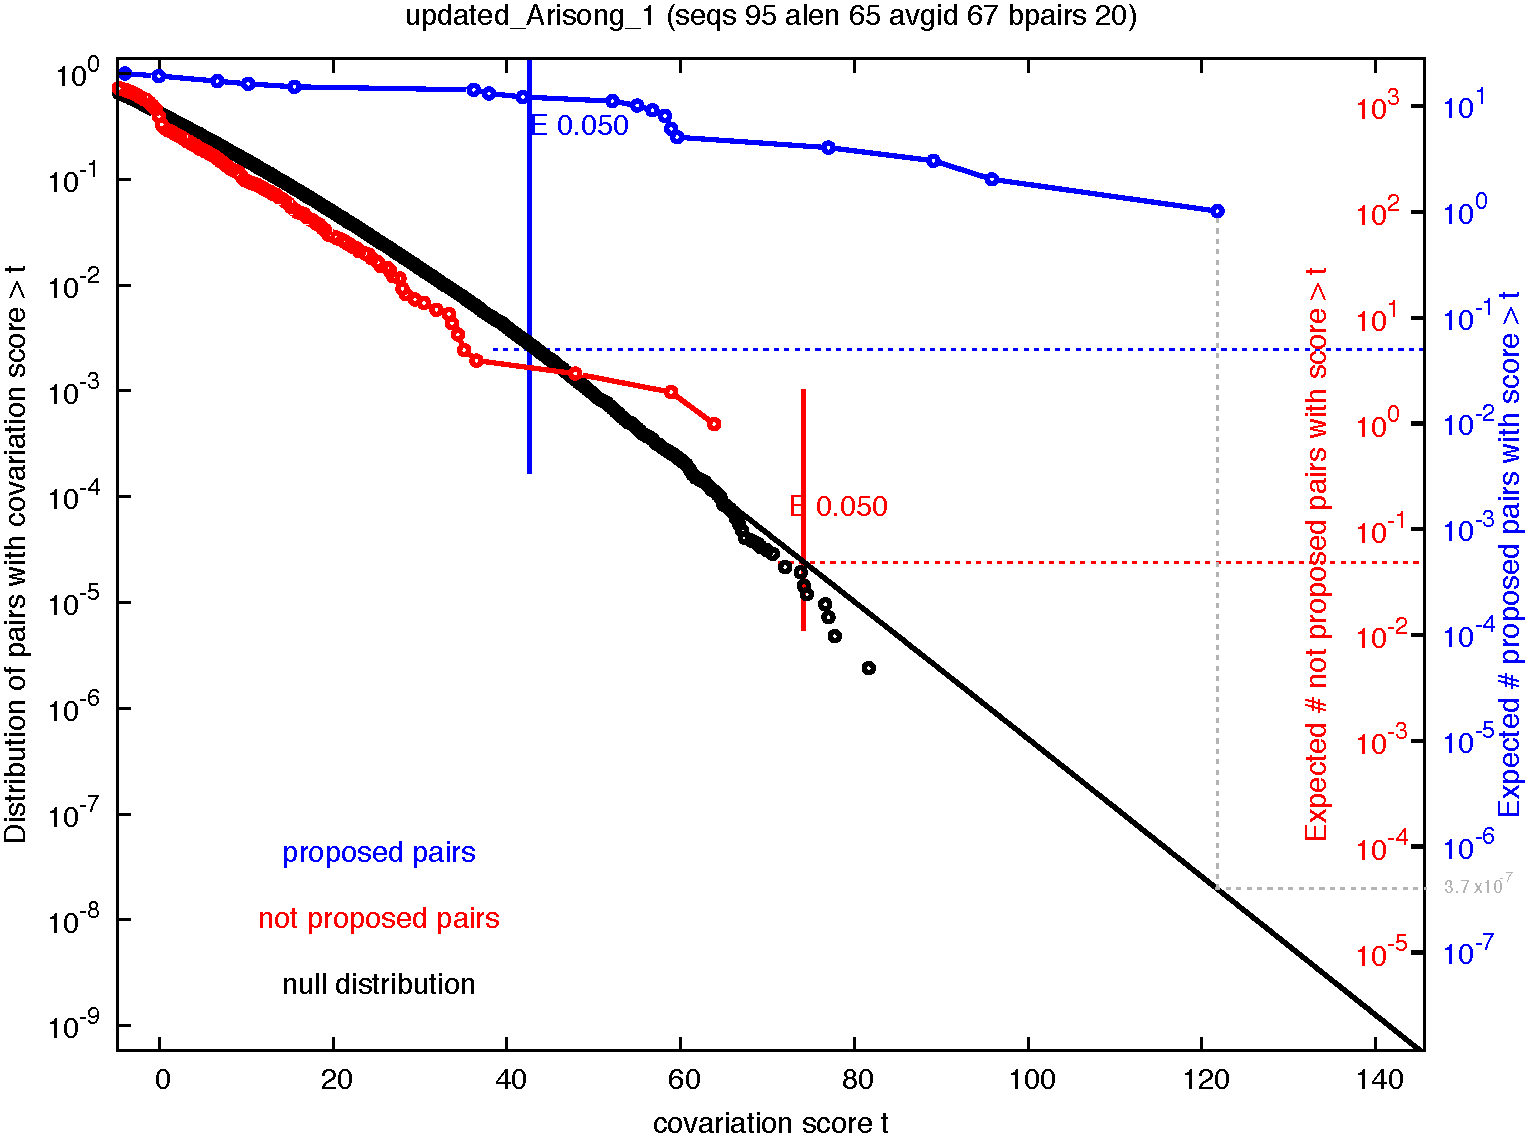
\includegraphics[scale=0.50]{Arisong_surv.pdf}
 \caption{\small\textbf{\emprog{tutorial/updated\_Arisong\_1.surv.\{ps,svg\}}:
 covariation scores survival function $P(X>x)$.}  The survival
 function of scores for all pairs in the given alignment is depicted
 in blue. The survival function for the null alignments is depicted in
 black. A black line indicates to fit to a truncated Gamma
 distribution of the tail of the null distribution. In red, we plot
 the survival function of scores for the pairs in the given alignment
 excluding those proposed as base pairs. For a particular pair, as an
 example the highest scoring one from the distribution of proposed
 pairs (blue), we obtain its E-value by drawing a vertical (gray) line
 from the point to the null distribution (black). The corresponding
 value in the blue scale gives us the E-value for that pair (in this
 example, 3.7 $\cdot$10$^{-7}$).
 }
 \label{fig:surv}
 \end{figure}

 \begin{figure}[h] 
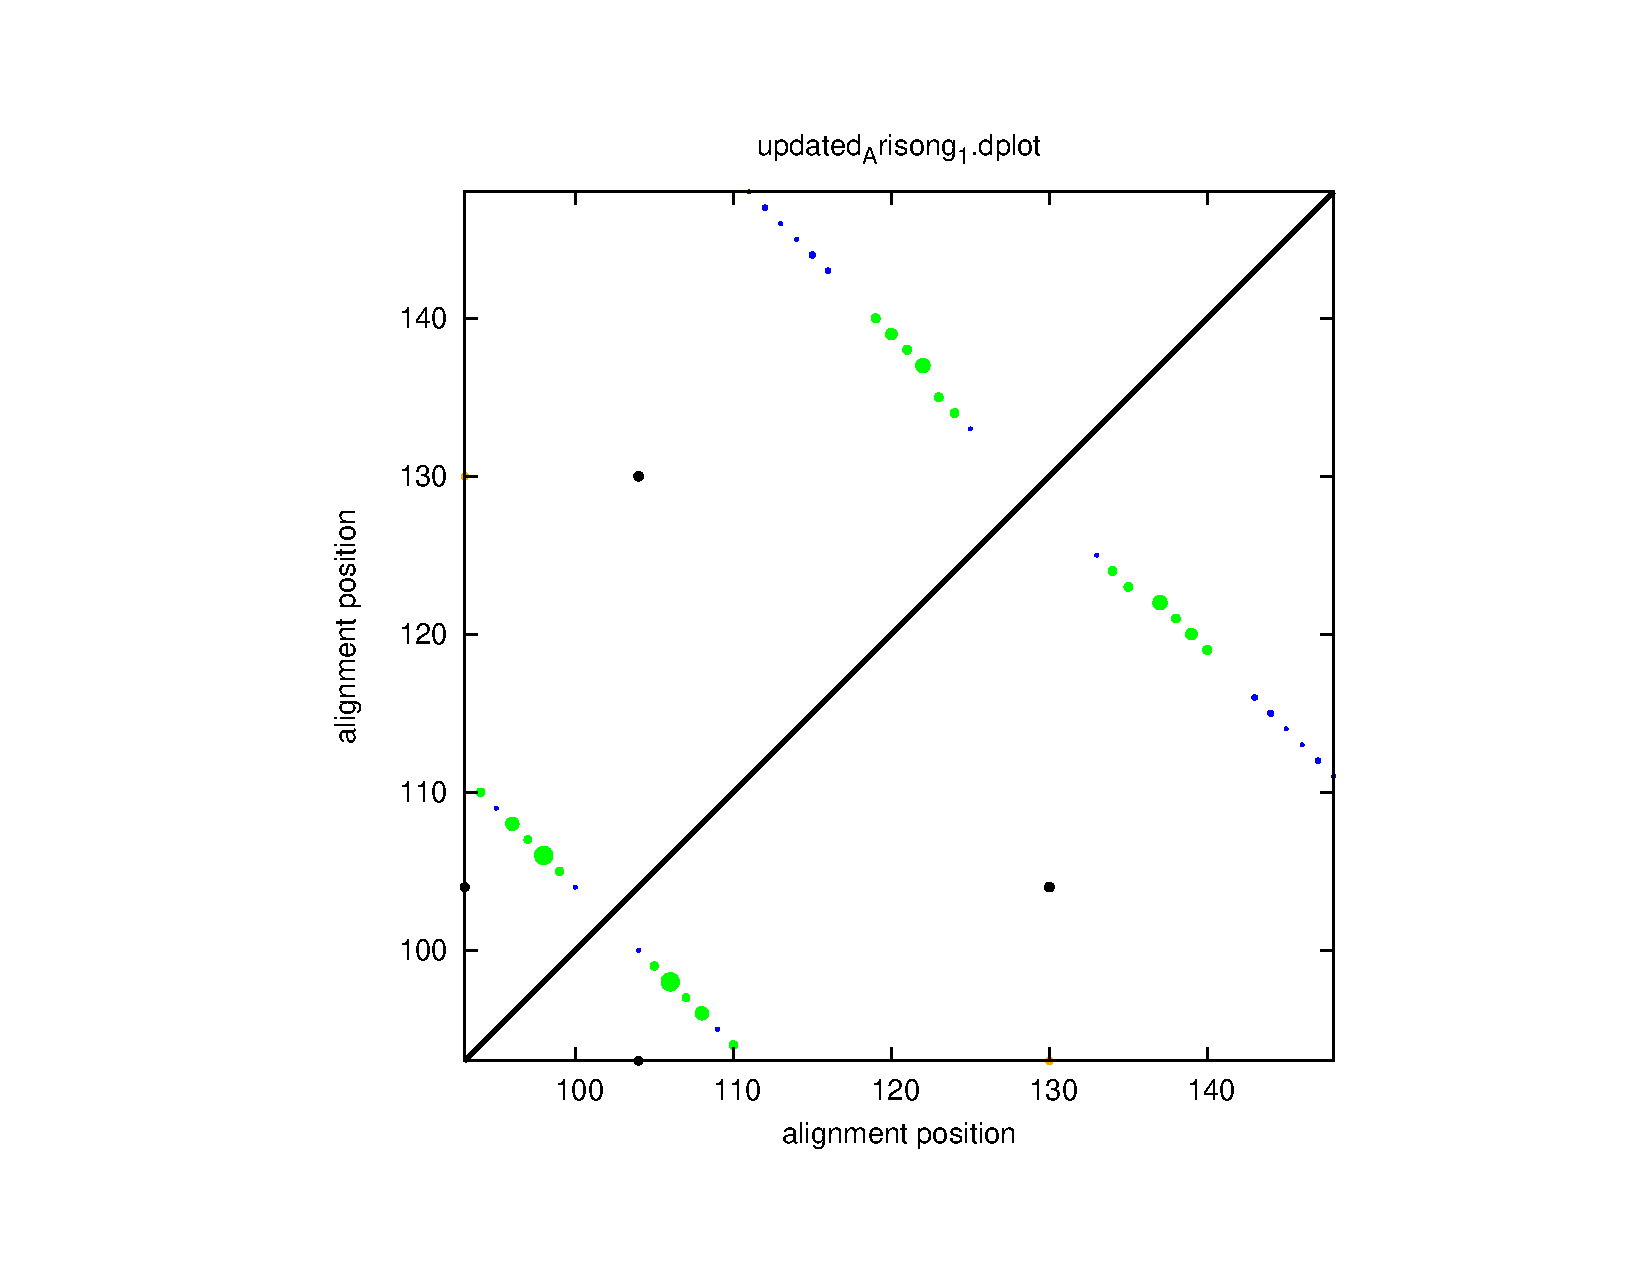
\includegraphics[scale=0.60]{Arisong_dplot.pdf} 
 \caption{\small\textbf{\emprog{tutorial/updated\_Arisong\_1.dplot.\{ps,svg\}}:
   dotplot.}  Dot size is proportional to the covariation score. In
   blue we depict the consensus base pairs; in green, the consensus
   base pairs that show significant covariation; in orange (none shown
   in this plot), we depict other pairs that have significant
   covariation, are not part of the consensus secondary structure but
   are compatible with it; in black we depict other significant pairs.
   Position are relative to the original input alignment (before any
   gapped column is removed).}
\label{fig:dplot} 
\end{figure}



 

